\chapter{Power Density \& Field Strength}
\label{ch:power-density-field-strength}

\begin{nontechnical}
\textbf{Power density is like measuring sunlight intensity}---how much energy hits each square meter. \textbf{Field strength} is like measuring the ``force'' of the electromagnetic wave at a point.

\textbf{Simple analogy:} Imagine standing near a campfire:
\begin{itemize}
\item \textbf{Field strength} = how hot the air feels on your skin
\item \textbf{Power density} = total heat energy hitting your body per square meter
\end{itemize}

\textbf{Real-world comparison:}
\begin{itemize}
\item \textbf{Sunlight:} 1000~W/m$^2$ (strong enough to power solar panels!)
\item \textbf{WiFi router @ 1~m:} 0.00001~W/m$^2$ (100 million times weaker)
\item \textbf{Cell tower @ 100~m:} 0.0001~W/m$^2$ (10 million times weaker)
\end{itemize}

\textbf{Key insight:} Double your distance from a source $\rightarrow$ you get $\frac{1}{4}$ the power density. This is why WiFi works at 50~m but not 200~m, and why satellites need enormous transmit power (they're 36,000~km away!).

\textbf{Safety:} FCC limits RF exposure to 10~W/m$^2$ for the general public. Typical WiFi and cell phone exposure is 1000--10,000 times below this limit.
\end{nontechnical}

\section{Overview}

\textbf{Power density} and \textbf{field strength} quantify the intensity of electromagnetic radiation at a given point in space. These fundamental parameters are essential for:

\begin{itemize}
\item \textbf{Link budget calculations:} Determine received signal strength
\item \textbf{Safety standards:} RF exposure limits (FCC, ICNIRP)
\item \textbf{Antenna performance:} Radiated power distribution
\item \textbf{Radar systems:} Detection capability vs distance
\item \textbf{EMC compliance:} Electromagnetic interference testing
\end{itemize}

\begin{keyconcept}
In the far field, power density $S$ is related to electric field strength $E$ by the fundamental relationship:
\[
S = \frac{E_{\text{rms}}^2}{377} \quad \text{(W/m}^2\text{)}
\]
where 377~$\Omega$ is the impedance of free space. Power density follows the \textbf{inverse square law}: $S \propto 1/r^2$.
\end{keyconcept}

\section{Mathematical Description}

\subsection{Electric Field Strength (E)}

The \textbf{electric field} $\vec{E}$ describes the force per unit charge exerted on a test charge:
\begin{equation}
\vec{E} = \frac{\vec{F}}{q}
\label{eq:efield-definition}
\end{equation}
where:
\begin{itemize}
\item $\vec{F}$ = force on test charge (N)
\item $q$ = test charge (coulombs)
\item Units: V/m or N/C (equivalent)
\end{itemize}

For an \textbf{electromagnetic wave} (plane wave propagating in $+z$ direction):
\begin{equation}
E(z,t) = E_0 \cos(\omega t - kz + \phi)
\label{eq:efield-wave}
\end{equation}
where:
\begin{itemize}
\item $E_0$ = peak electric field amplitude (V/m)
\item $\omega = 2\pi f$ = angular frequency (rad/s)
\item $k = 2\pi/\lambda$ = wave number (rad/m)
\item $\phi$ = phase offset (rad)
\end{itemize}

\textbf{RMS (Root Mean Square) value:}
\begin{equation}
E_{\text{rms}} = \frac{E_0}{\sqrt{2}}
\label{eq:efield-rms}
\end{equation}

Most field strength specifications use RMS values for consistency with power calculations.

\subsubsection{Typical Field Strength Values}

\begin{center}
\begin{tabular}{@{}lll@{}}
\toprule
Source & Distance & E-field (V/m) \\
\midrule
AM broadcast (50~kW) & 1~km & $\sim$0.1 \\
FM broadcast (100~kW) & 1~km & $\sim$0.2 \\
Cell tower (40~W ERP) & 100~m & $\sim$1--2 \\
WiFi router (100~mW) & 1~m & $\sim$3 \\
Microwave oven leak & 5~cm & $\sim$10--50 (max allowed) \\
Lightning & Near channel & $\sim$10$^6$ \\
\bottomrule
\end{tabular}
\end{center}

\subsection{Magnetic Field Strength (H)}

The \textbf{magnetic field strength} $\vec{H}$ describes the magnetizing force:
\begin{equation}
\vec{H} = \frac{\vec{B}}{\mu}
\label{eq:hfield-definition}
\end{equation}
where:
\begin{itemize}
\item $\vec{B}$ = magnetic flux density (Tesla or Wb/m$^2$)
\item $\mu$ = permeability (H/m)
\item Units: A/m (amperes per meter)
\end{itemize}

In free space:
\begin{equation}
\mu_0 = 4\pi \times 10^{-7} \approx 1.257 \times 10^{-6} \text{~H/m}
\label{eq:permeability-free-space}
\end{equation}

\subsection{E-H Relationship in Far Field}

In a \textbf{plane wave} (far from the source), the electric and magnetic fields are related by the \textbf{wave impedance of free space}:
\begin{equation}
\frac{E}{H} = \eta_0 = \sqrt{\frac{\mu_0}{\epsilon_0}} = 120\pi \approx 377~\Omega
\label{eq:wave-impedance}
\end{equation}
where:
\begin{itemize}
\item $\eta_0$ = impedance of free space ($\approx$377~$\Omega$)
\item $\epsilon_0 = 8.854 \times 10^{-12}$~F/m = permittivity of free space
\end{itemize}

\textbf{Practical conversion:}
\begin{equation}
H = \frac{E}{377} \quad \text{(A/m)}
\label{eq:h-from-e}
\end{equation}

\textbf{Example:} For $E = 10$~V/m, the magnetic field strength is:
\[
H = \frac{10}{377} \approx 0.0265 \text{~A/m}
\]

\subsection{Electromagnetic Wave Visualization}

\begin{center}
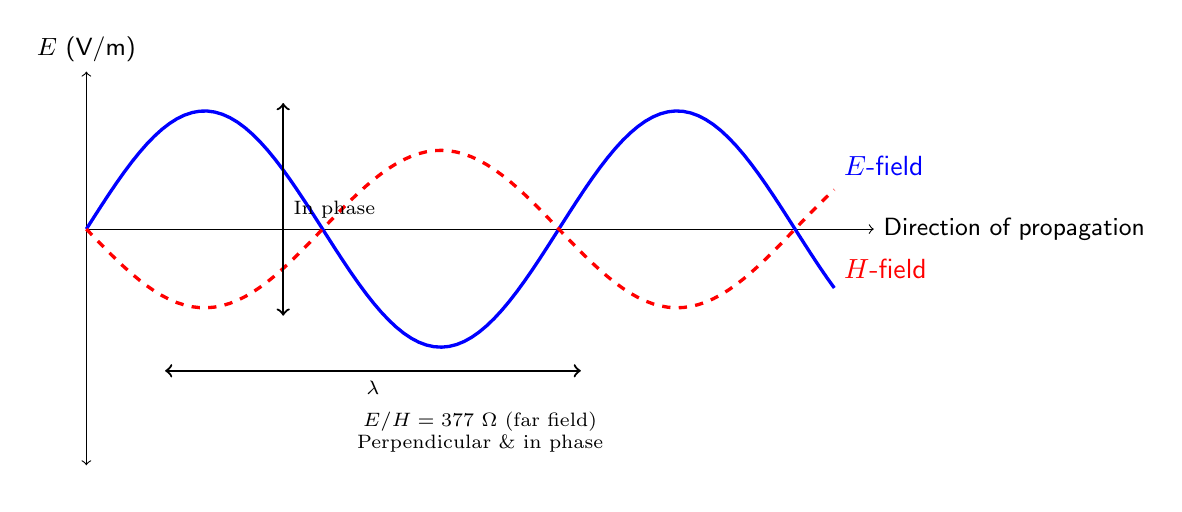
\begin{tikzpicture}[scale=1.0]
% Axes
\draw[->] (0,0) -- (10,0) node[right] {\sffamily\small Direction of propagation};
\draw[->] (0,-2) -- (0,2) node[above] {\sffamily\small $E$ (V/m)};
\draw[->] (0,0) -- (0,-3) node[below] {};

% Electric field wave (vertical)
\draw[very thick, blue] plot[domain=0:9.5, samples=100] (\x, {1.5*sin(\x*60)});
\node[blue, right] at (9.5, 0.8) {\sffamily $E$-field};

% Magnetic field wave (into/out of page, shown as perpendicular)
\draw[very thick, red, dashed] plot[domain=0:9.5, samples=100] (\x, {-1.0*sin(\x*60)});
\node[red, right] at (9.5, -0.5) {\sffamily $H$-field};

% Phase relationship annotation
\draw[<->, thick] (2.5, 1.6) -- (2.5, -1.1) node[midway, right, font=\scriptsize] {In phase};
\node[below, font=\scriptsize, align=center] at (5, -2.2) {$E/H = 377~\Omega$ (far field)\\Perpendicular \& in phase};

% Wavelength annotation
\draw[<->, thick] (1, -1.8) -- (6.28, -1.8) node[midway, below, font=\scriptsize] {$\lambda$};
\end{tikzpicture}
\end{center}

\subsection{Near Field vs Far Field}

The electromagnetic field around an antenna is divided into distinct regions with different characteristics.

\subsubsection{Near Field (Reactive Near Field)}

\textbf{Distance from antenna:}
\begin{equation}
r < 0.62\sqrt{\frac{D^3}{\lambda}} \quad \text{(large antennas)}
\label{eq:near-field-distance}
\end{equation}
or for small antennas:
\begin{equation}
r < \frac{\lambda}{2\pi}
\label{eq:near-field-small}
\end{equation}
where:
\begin{itemize}
\item $D$ = largest antenna dimension (m)
\item $\lambda$ = wavelength (m)
\end{itemize}

\textbf{Characteristics:}
\begin{itemize}
\item $E/H \neq 377~\Omega$ (reactive energy dominates)
\item Energy oscillates between E-field and H-field storage
\item Fields decay faster than $1/r$ (typically $1/r^2$ or $1/r^3$)
\item Inductive or capacitive coupling dominates
\end{itemize}

\subsubsection{Far Field (Radiating Far Field)}

\textbf{Distance from antenna (Fraunhofer distance):}
\begin{equation}
r > \frac{2D^2}{\lambda}
\label{eq:far-field-distance}
\end{equation}

\textbf{Characteristics:}
\begin{itemize}
\item $E/H = 377~\Omega$ (plane wave approximation valid)
\item Radiation pattern independent of distance (shape constant)
\item Fields decay as $1/r$, power density as $1/r^2$
\item This is where link budget calculations apply
\end{itemize}

\begin{calloutbox}{Example: WiFi Far Field Boundary}
\textbf{Given:} WiFi 2.4~GHz ($\lambda = 12.5$~cm), antenna size $D = 5$~cm

\textbf{Solution:}
\[
r_{\text{far}} = \frac{2 \times (0.05)^2}{0.125} = \frac{0.005}{0.125} = 0.04 \text{~m} = 4 \text{~cm}
\]

\textbf{Result:} Far field begins at only 4~cm from the antenna. This is why most WiFi communications operate in the far field region.
\end{calloutbox}

\subsection{Field Regions Visualization}

\begin{center}
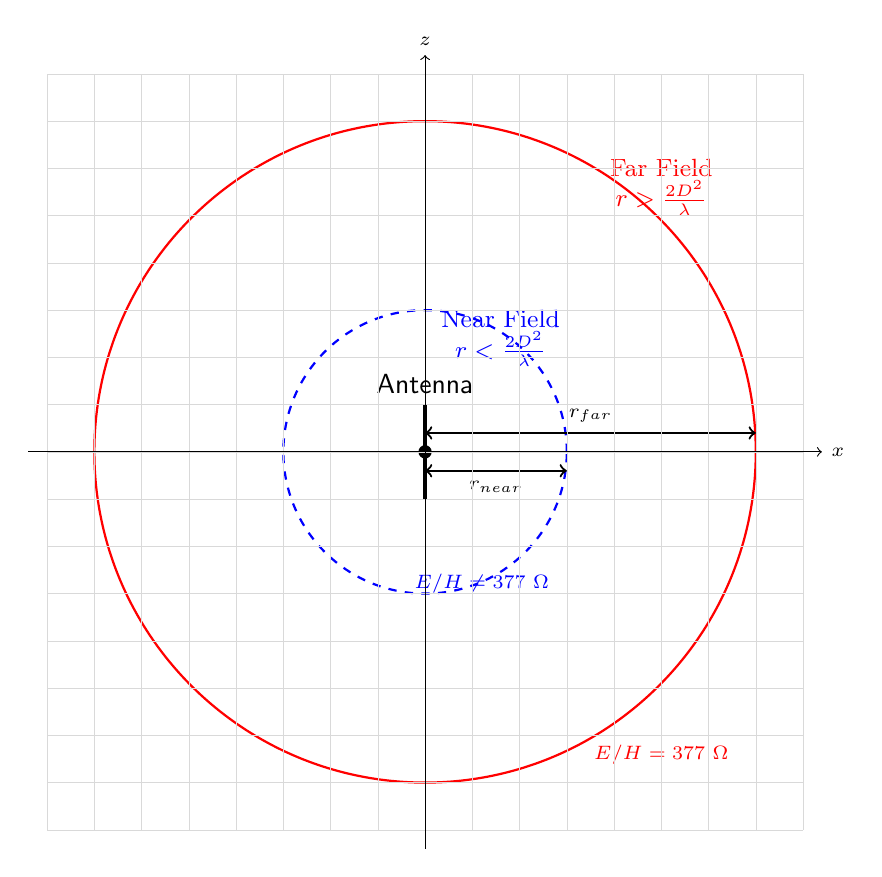
\begin{tikzpicture}[scale=1.2]
% Antenna
\draw[very thick] (0, -0.5) -- (0, 0.5) node[above] {\sffamily Antenna};
\fill[black] (0,0) circle (2pt);

% Near field region
\draw[thick, blue, dashed] (0,0) circle (1.5);
\node[blue, align=center, font=\small] at (0.8, 1.2) {Near Field\\$r < \frac{2D^2}{\lambda}$};
\node[blue, font=\scriptsize] at (0.6, -1.4) {$E/H \neq 377~\Omega$};

% Far field region
\draw[thick, red] (0,0) circle (3.5);
\node[red, align=center, font=\small] at (2.5, 2.8) {Far Field\\$r > \frac{2D^2}{\lambda}$};
\node[red, font=\scriptsize] at (2.5, -3.2) {$E/H = 377~\Omega$};

% Distance annotations
\draw[<->, thick] (0, -0.2) -- (1.5, -0.2) node[midway, below, font=\scriptsize] {$r_{\text{near}}$};
\draw[<->, thick] (0, 0.2) -- (3.5, 0.2) node[midway, above, font=\scriptsize] {$r_{\text{far}}$};

% Grid for reference
\draw[very thin, gray!30] (-4, -4) grid[step=0.5] (4, 4);
\draw[->] (-4.2, 0) -- (4.2, 0) node[right, font=\scriptsize] {$x$};
\draw[->] (0, -4.2) -- (0, 4.2) node[above, font=\scriptsize] {$z$};
\end{tikzpicture}
\end{center}

\section{Power Density and Poynting Vector}

\subsection{The Poynting Vector}

The \textbf{Poynting vector} $\vec{S}$ represents power flow per unit area:
\begin{equation}
\vec{S} = \vec{E} \times \vec{H}
\label{eq:poynting-vector}
\end{equation}
where:
\begin{itemize}
\item $\vec{S}$ = power density vector (W/m$^2$)
\item $\vec{E}$ = electric field vector (V/m)
\item $\vec{H}$ = magnetic field vector (A/m)
\item Direction: direction of energy propagation
\end{itemize}

For a plane wave with $\vec{E} \perp \vec{H}$, the magnitude is:
\begin{equation}
S = E \cdot H = \frac{E^2}{\eta_0} = \frac{E^2}{377}
\label{eq:power-density-e}
\end{equation}

Alternatively, in terms of magnetic field:
\begin{equation}
S = \eta_0 H^2 = 377 H^2
\label{eq:power-density-h}
\end{equation}

\subsection{Time-Averaged Power Density}

For a sinusoidal wave, instantaneous power oscillates at $2f$. The \textbf{time-averaged} power density is:
\begin{equation}
\langle S \rangle = \frac{1}{2} \frac{E_0^2}{\eta_0} = \frac{E_{\text{rms}}^2}{\eta_0} = \frac{E_{\text{rms}}^2}{377}
\label{eq:power-density-rms}
\end{equation}
where:
\begin{itemize}
\item $E_0$ = peak electric field amplitude (V/m)
\item $E_{\text{rms}} = E_0/\sqrt{2}$ = RMS electric field (V/m)
\end{itemize}

\textbf{Example:} For $E_{\text{rms}} = 10$~V/m:
\[
\langle S \rangle = \frac{100}{377} \approx 0.265 \text{~W/m}^2
\]

\section{Inverse Square Law}

\subsection{Power Density from Isotropic Source}

An \textbf{isotropic radiator} distributes power uniformly over a spherical surface:
\begin{equation}
S = \frac{P_t}{4\pi r^2}
\label{eq:inverse-square-law}
\end{equation}
where:
\begin{itemize}
\item $P_t$ = transmitted power (W)
\item $r$ = distance from source (m)
\item $4\pi r^2$ = surface area of sphere (m$^2$)
\end{itemize}

This is the fundamental \textbf{inverse square law}: power density decreases as $1/r^2$.

\begin{calloutbox}{Example: Isotropic Source}
\textbf{Given:} 100~W isotropic source at 10~m distance

\textbf{Solution:}
\[
S = \frac{100}{4\pi (10)^2} = \frac{100}{1257} \approx 0.0796 \text{~W/m}^2
\]

\textbf{At 20~m} (double the distance):
\[
S = \frac{100}{4\pi (20)^2} = \frac{100}{5027} \approx 0.0199 \text{~W/m}^2
\]

\textbf{Result:} Doubling distance reduces power density by $\frac{1}{4}$ (6~dB reduction).
\end{calloutbox}

\subsection{Inverse Square Law Visualization}

\begin{center}
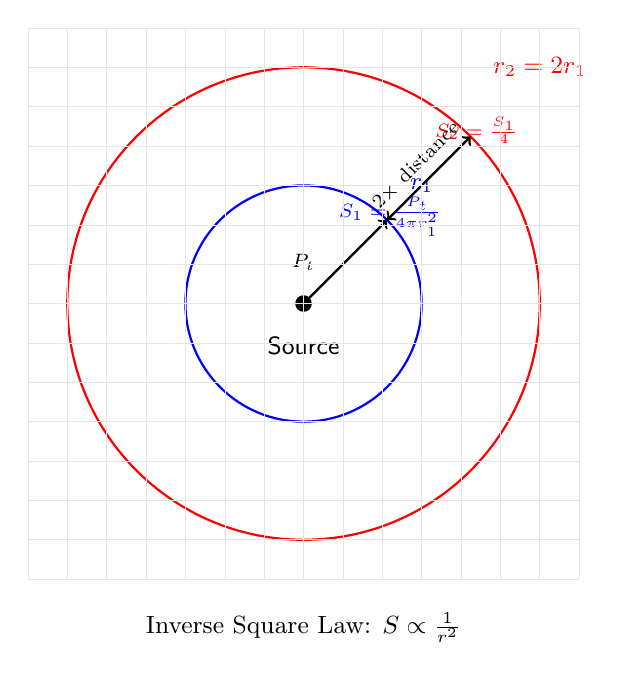
\begin{tikzpicture}[scale=1.0]
% Source
\fill[black] (0,0) circle (3pt);
\node[below] at (0, -0.3) {\sffamily\small Source};
\node[above, font=\scriptsize] at (0, 0.3) {$P_t$};

% Spheres at different distances
\draw[thick, blue] (0,0) circle (1.5);
\node[blue, font=\small] at (1.5, 1.5) {$r_1$};
\node[blue, font=\scriptsize, align=center] at (1.1, 1.1) {$S_1 = \frac{P_t}{4\pi r_1^2}$};

\draw[thick, red] (0,0) circle (3.0);
\node[red, font=\small] at (3.0, 3.0) {$r_2 = 2r_1$};
\node[red, font=\scriptsize, align=center] at (2.2, 2.2) {$S_2 = \frac{S_1}{4}$};

% Radial lines
\draw[->, thick] (0,0) -- (45:1.5) node[midway, above, sloped, font=\scriptsize] {};
\draw[->, thick] (0,0) -- (45:3.0);

% Power density indicators
\draw[<->, thick] (45:1.5) -- (45:3.0) node[midway, above, sloped, font=\scriptsize] {$2\times$ distance};

% Grid reference
\draw[very thin, gray!20] (-3.5, -3.5) grid[step=0.5] (3.5, 3.5);

% Annotations
\node[below, font=\small, align=center] at (0, -3.8) {Inverse Square Law: $S \propto \frac{1}{r^2}$};
\end{tikzpicture}
\end{center}

\subsection{Power Density from Directional Antenna}

An antenna with gain $G$ concentrates power in a preferred direction:
\begin{equation}
S = \frac{P_t \cdot G}{4\pi r^2}
\label{eq:power-density-gain}
\end{equation}

The \textbf{Effective Isotropic Radiated Power (EIRP)} is defined as:
\begin{equation}
\text{EIRP} = P_t \cdot G
\label{eq:eirp}
\end{equation}
where:
\begin{itemize}
\item $P_t$ = transmitter power (W)
\item $G$ = antenna gain (linear, not dB)
\end{itemize}

Substituting EIRP:
\begin{equation}
S = \frac{\text{EIRP}}{4\pi r^2}
\label{eq:power-density-eirp}
\end{equation}

\begin{warningbox}
\textbf{CRITICAL:} Antenna gain must be in \textbf{linear units}, not dB. Convert from dBi using:
\[
G_{\text{linear}} = 10^{G_{\text{dBi}}/10}
\]
For example, 2~dBi = $10^{0.2} \approx 1.58$ (linear).
\end{warningbox}

\begin{calloutbox}{Example: WiFi Router Power Density}
\textbf{Given:}
\begin{itemize}
\item Transmit power: $P_t = 100$~mW = 0.1~W
\item Antenna gain: 2~dBi (linear gain $\approx 1.58$)
\item Distance: $r = 10$~m
\end{itemize}

\textbf{Solution:}

\textbf{Step 1:} Calculate EIRP
\[
\text{EIRP} = 0.1 \times 1.58 = 0.158 \text{~W}
\]

\textbf{Step 2:} Calculate power density
\[
S = \frac{0.158}{4\pi (10)^2} = \frac{0.158}{1257} \approx 0.000126 \text{~W/m}^2 = 0.126 \text{~mW/m}^2
\]

\textbf{Step 3:} Convert to E-field
\[
E_{\text{rms}} = \sqrt{S \times 377} = \sqrt{0.000126 \times 377} \approx 0.218 \text{~V/m}
\]

\textbf{Result:} At 10~m from a typical WiFi router, the power density is 0.126~mW/m$^2$ and the E-field strength is 0.22~V/m---both well below safety limits.
\end{calloutbox}

\section{Conversion Formulas}

\subsection{Power Density to Electric Field}

Summary formulas for far-field plane waves:

\textbf{Power density from E-field:}
\begin{equation}
S = \frac{E_{\text{rms}}^2}{377} \quad \text{(W/m}^2\text{)}
\label{eq:s-from-e-conversion}
\end{equation}

\textbf{E-field from power density:}
\begin{equation}
E_{\text{rms}} = \sqrt{377 \times S} \approx 19.4\sqrt{S} \quad \text{(V/m)}
\label{eq:e-from-s-conversion}
\end{equation}

\textbf{Peak E-field:}
\begin{equation}
E_0 = \sqrt{2} \times E_{\text{rms}} = \sqrt{2 \times 377 \times S} \approx 27.5\sqrt{S}
\label{eq:e-peak-from-s}
\end{equation}

\subsection{Quick Conversion Reference}

\begin{center}
\begin{tabular}{@{}lll@{}}
\toprule
Power Density (W/m$^2$) & $E_{\text{rms}}$ (V/m) & $E_{\text{peak}}$ (V/m) \\
\midrule
0.001 (1~mW/m$^2$) & 0.61 & 0.87 \\
0.01 (10~mW/m$^2$) & 1.94 & 2.75 \\
0.1 & 6.14 & 8.68 \\
1 & 19.4 & 27.5 \\
10 & 61.4 & 86.8 \\
100 & 194 & 275 \\
\bottomrule
\end{tabular}
\end{center}

\section{Power Delivered to Receiving Antenna}

\subsection{Effective Aperture}

The \textbf{effective aperture} $A_e$ of an antenna captures power from an incident electromagnetic wave:
\begin{equation}
P_r = S \cdot A_e
\label{eq:received-power-aperture}
\end{equation}
where:
\begin{itemize}
\item $P_r$ = received power (W)
\item $S$ = power density (W/m$^2$)
\item $A_e$ = effective aperture (m$^2$)
\end{itemize}

The effective aperture is related to antenna gain by:
\begin{equation}
A_e = \frac{G_r \lambda^2}{4\pi}
\label{eq:effective-aperture}
\end{equation}
where:
\begin{itemize}
\item $G_r$ = receive antenna gain (linear)
\item $\lambda$ = wavelength (m)
\end{itemize}

\subsection{Friis Transmission Equation}

Combining the power density formula with effective aperture:
\begin{equation}
P_r = \frac{P_t G_t G_r \lambda^2}{(4\pi r)^2}
\label{eq:friis-equation}
\end{equation}
where:
\begin{itemize}
\item $P_t$ = transmit power (W)
\item $G_t$ = transmit antenna gain (linear)
\item $G_r$ = receive antenna gain (linear)
\item $r$ = distance between antennas (m)
\end{itemize}

This is the famous \textbf{Friis transmission equation}. See Chapter~\ref{ch:fspl} for detailed link budget analysis.

\section{Worked Example: Satellite Downlink}

\begin{calloutbox}{Complete Link Budget Calculation}
\textbf{Problem:} Calculate the power density, E-field strength, and received power for a geostationary satellite downlink.

\textbf{Given:}
\begin{itemize}
\item Satellite EIRP: 50~dBW = 100~kW
\item Frequency: 12~GHz ($\lambda = 0.025$~m)
\item Distance: 36,000~km (GEO orbit)
\item RX antenna: 1~m$^2$ dish (gain $\approx$ 40~dBi = 10,000 linear)
\item Effective aperture: $A_e \approx 0.5$~m$^2$ (typical efficiency)
\end{itemize}

\textbf{Solution:}

\textbf{Step 1:} Power density at ground
\[
S = \frac{\text{EIRP}}{4\pi r^2} = \frac{10^5}{4\pi (3.6 \times 10^7)^2} = \frac{10^5}{1.63 \times 10^{16}} \approx 6.1 \times 10^{-12} \text{~W/m}^2
\]

\textbf{Step 2:} E-field strength
\[
E_{\text{rms}} = \sqrt{377 \times S} = \sqrt{377 \times 6.1 \times 10^{-12}} \approx 1.5 \times 10^{-3} \text{~V/m} = 1.5 \text{~mV/m}
\]

\textbf{Step 3:} Received power (using aperture method)
\[
P_r = S \cdot A_e = 6.1 \times 10^{-12} \times 0.5 \approx 3 \times 10^{-12} \text{~W} = 3 \text{~pW}
\]

In dBm:
\[
P_r(\text{dBm}) = 10\log_{10}\left(\frac{3 \times 10^{-12}}{10^{-3}}\right) = -115 \text{~dBm}
\]

\textbf{Step 4:} Verify using Friis equation
\[
P_r = \frac{P_t G_t G_r \lambda^2}{(4\pi r)^2} = \frac{100{,}000 \times 1 \times 10{,}000 \times (0.025)^2}{(4\pi \times 3.6 \times 10^7)^2} \approx 3 \times 10^{-12} \text{~W}
\]

\textbf{Result:} Both methods give $\approx$3~pW or $-115$~dBm. This is consistent and shows the extremely weak signal from a geostationary satellite requires sensitive receivers and low-noise amplifiers.
\end{calloutbox}

\section{RF Safety Standards}

Exposure limits protect against thermal and non-thermal effects from electromagnetic radiation.

\subsection{FCC Limits (USA)}

\subsubsection{Occupational/Controlled Exposure}

For workers aware of RF exposure:

\begin{center}
\begin{tabular}{@{}llll@{}}
\toprule
Frequency & E-field (V/m) & H-field (A/m) & Power Density (W/m$^2$) \\
\midrule
0.3--3~MHz & 614 & 1.63 & --- \\
3--30~MHz & $1842/f$ & $4.89/f$ & --- \\
30--300~MHz & 61.4 & 0.163 & 1.0 \\
300--1500~MHz & --- & --- & $f/300$ \\
1500--100,000~MHz & --- & --- & 5.0 \\
\bottomrule
\end{tabular}
\end{center}

where $f$ is in MHz.

\subsubsection{General Population/Uncontrolled Exposure}

For the general public, limits are \textbf{5$\times$ lower} than occupational limits. For example:
\begin{itemize}
\item 30--300~MHz: 0.2~W/m$^2$ (vs 1.0~W/m$^2$ occupational)
\item 1500--100,000~MHz: 1.0~W/m$^2$ (vs 5.0~W/m$^2$ occupational)
\end{itemize}

\subsection{ICNIRP Limits (International)}

For general public (6-minute average):

\begin{center}
\begin{tabular}{@{}lll@{}}
\toprule
Frequency & E-field (V/m) & Power Density (W/m$^2$) \\
\midrule
10--400~MHz & 28 & 2 \\
400--2000~MHz & $1.375\sqrt{f}$ & $f/200$ \\
2--300~GHz & 61 & 10 \\
\bottomrule
\end{tabular}
\end{center}

where $f$ is in MHz.

\begin{calloutbox}{Example: WiFi Router Compliance Check}
\textbf{Given:} WiFi 2.4~GHz, 100~mW transmit power, 2~dBi gain

\textbf{Question:} Is it safe at 20~cm from a person (typical distance)?

\textbf{Solution:}

\textbf{Step 1:} Calculate power density at 20~cm
\[
S = \frac{P_t \cdot G}{4\pi r^2} = \frac{0.1 \times 1.58}{4\pi (0.2)^2} = \frac{0.158}{0.503} \approx 0.314 \text{~W/m}^2
\]

\textbf{Step 2:} Compare to limits
\begin{itemize}
\item \textbf{FCC limit @ 2.4~GHz:} 1.0~W/m$^2$ (uncontrolled), 5.0~W/m$^2$ (controlled)
\item \textbf{ICNIRP limit:} $f/200 = 2400/200 = 12$~W/m$^2$
\end{itemize}

\textbf{Step 3:} Safety margin
\[
\text{Margin} = \frac{1.0}{0.314} \approx 3.2 \quad (5~\text{dB})
\]

\textbf{Result:} At 20~cm, power density is 0.314~W/m$^2$ $<$ 1~W/m$^2$ (FCC limit). The router complies, but with only 5~dB margin.

\textbf{At 1~m:} $S = 0.0126$~W/m$^2$ (much safer, 19~dB margin).
\end{calloutbox}

\section{Applications}

\subsection{Radar Power Budget}

The \textbf{radar equation} relates transmitted power to received echo power:
\begin{equation}
P_r = \frac{P_t G^2 \lambda^2 \sigma}{(4\pi)^3 R^4}
\label{eq:radar-equation}
\end{equation}
where:
\begin{itemize}
\item $\sigma$ = target radar cross-section (m$^2$)
\item $R$ = range to target (m)
\item $G$ = antenna gain (same for transmit and receive)
\end{itemize}

Power density at target:
\begin{equation}
S_{\text{target}} = \frac{P_t G}{4\pi R^2}
\label{eq:power-density-target}
\end{equation}

Reflected power density back at radar:
\begin{equation}
S_{\text{return}} = \frac{S_{\text{target}} \cdot \sigma}{4\pi R^2} = \frac{P_t G \sigma}{(4\pi)^2 R^4}
\label{eq:power-density-return}
\end{equation}

\textbf{Note:} The $1/R^4$ dependence arises because power travels to the target and back ($1/R^2$ each way).

\begin{calloutbox}{Example: Weather Radar}
\textbf{Given:}
\begin{itemize}
\item Transmit power: $P_t = 1$~MW (peak)
\item Antenna gain: 45~dBi ($\approx$ 31,600 linear)
\item Frequency: 3~GHz ($\lambda = 0.1$~m)
\item Target: Raindrop, $\sigma = 10^{-6}$~m$^2$ (light rain)
\item Range: $R = 100$~km
\end{itemize}

\textbf{Solution:}

\textbf{Step 1:} Power density at raindrop
\[
S_{\text{target}} = \frac{10^6 \times 31{,}600}{4\pi (10^5)^2} = \frac{3.16 \times 10^{10}}{1.26 \times 10^{11}} \approx 0.25 \text{~W/m}^2
\]

\textbf{Step 2:} Received echo power
\[
P_r = \frac{10^6 \times (31{,}600)^2 \times (0.1)^2 \times 10^{-6}}{(4\pi)^3 (10^5)^4} \approx 1.6 \times 10^{-13} \text{~W} = -98 \text{~dBm}
\]

\textbf{Result:} Echo power is $-98$~dBm, weak but detectable with a sensitive receiver (typical noise floor $\sim$$-110$~dBm).
\end{calloutbox}

\subsection{Electromagnetic Interference (EMI)}

Field strength limits for conducted and radiated emissions are critical for electromagnetic compatibility (EMC).

\subsubsection{FCC Part 15 Radiated Emission Limits}

Class B limits (residential use):

\begin{center}
\begin{tabular}{@{}lll@{}}
\toprule
Frequency & E-field @ 3~m ($\mu$V/m) & dB$\mu$V/m \\
\midrule
30--88~MHz & 100 & 40 \\
88--216~MHz & 150 & 43.5 \\
216--960~MHz & 200 & 46 \\
Above 960~MHz & 500 & 54 \\
\bottomrule
\end{tabular}
\end{center}

\textbf{Measurement method:} Use calibrated antenna + spectrum analyzer at specified distance.

\begin{calloutbox}{Example: Spurious Emission Check}
\textbf{Given:} Digital device @ 300~MHz, measured 180~$\mu$V/m @ 3~m

\textbf{Limit @ 300~MHz:} 200~$\mu$V/m

\textbf{Result:} $180 < 200$ $\rightarrow$ \textbf{Pass}

\textbf{Margin:} $20\log_{10}(200/180) = 0.9$~dB (minimal margin)
\end{calloutbox}

\subsection{Field Strength in Different Media}

In a dielectric medium (not free space), the wave impedance changes:
\begin{equation}
\eta = \sqrt{\frac{\mu}{\epsilon}} = \frac{\eta_0}{\sqrt{\epsilon_r}}
\label{eq:impedance-dielectric}
\end{equation}
where:
\begin{itemize}
\item $\epsilon_r$ = relative permittivity
\item $\eta_0 = 377~\Omega$ (free space)
\end{itemize}

\textbf{Example:} Water ($\epsilon_r \approx 80$ @ low frequencies)
\[
\eta_{\text{water}} = \frac{377}{\sqrt{80}} \approx 42~\Omega
\]

Power density for same E-field:
\[
S = \frac{E^2}{42}
\]

This is \textbf{9$\times$ higher power density} than free space for the same E-field strength.

\textbf{Implication:} Underwater communications require different impedance matching than air/vacuum systems.

\subsection{Antenna Gain and Directivity}

Antenna gain increases power density in a preferred direction:
\begin{equation}
G = \eta_{\text{ant}} \cdot D
\label{eq:antenna-gain}
\end{equation}
where:
\begin{itemize}
\item $\eta_{\text{ant}}$ = antenna efficiency (0--1)
\item $D$ = directivity (ratio of max to average power density)
\end{itemize}

Directivity is defined as:
\begin{equation}
D = \frac{S_{\text{max}}}{S_{\text{avg}}} = \frac{4\pi S_{\text{max}} r^2}{P_t}
\label{eq:directivity}
\end{equation}

\textbf{Common antennas:}
\begin{itemize}
\item \textbf{Isotropic antenna:} $D = 1$ (0~dBi) --- power uniformly distributed
\item \textbf{Half-wave dipole:} $D = 1.64$ (2.15~dBi) --- power concentrated in broadside direction
\item \textbf{Parabolic dish:} For diameter $D_{\text{ant}}$ and wavelength $\lambda$:
\end{itemize}
\begin{equation}
G \approx \eta_{\text{ant}} \left(\frac{\pi D_{\text{ant}}}{\lambda}\right)^2
\label{eq:parabolic-gain}
\end{equation}
with $\eta_{\text{ant}} \approx 0.5$--0.7 (typical).

\subsection{Skin Depth and Field Penetration}

In conductors, the electric field decays exponentially:
\begin{equation}
E(z) = E_0 e^{-z/\delta}
\label{eq:skin-effect}
\end{equation}

The \textbf{skin depth} $\delta$ is:
\begin{equation}
\delta = \sqrt{\frac{2}{\omega \mu \sigma}} = \sqrt{\frac{1}{\pi f \mu \sigma}}
\label{eq:skin-depth}
\end{equation}
where:
\begin{itemize}
\item $\sigma$ = conductivity (S/m)
\item $f$ = frequency (Hz)
\item For copper: $\sigma = 5.8 \times 10^7$~S/m
\end{itemize}

\textbf{Example:} Copper @ 1~GHz
\[
\delta = \sqrt{\frac{1}{\pi \times 10^9 \times 4\pi \times 10^{-7} \times 5.8 \times 10^7}} \approx 2.1~\mu\text{m}
\]

\textbf{Implication:} At microwave frequencies, current flows in a very thin surface layer ($<$ 2~$\mu$m), which increases conductor resistance and loss.

\section{Summary}

\subsection{Key Parameters}

\begin{center}
\begin{tabular}{@{}lllll@{}}
\toprule
Quantity & Symbol & Units & Typical Range & Key Relationship \\
\midrule
Electric field & $E$ & V/m & 0.01--1000 & $E = \sqrt{377 \times S}$ \\
Magnetic field & $H$ & A/m & 0.00003--3 & $H = E/377$ \\
Power density & $S$ & W/m$^2$ & $10^{-6}$--10 & $S = E^2/377$ \\
Transmit power & $P_t$ & W & 0.001--100,000 & $S = P_t G / (4\pi r^2)$ \\
Distance & $r$ & m & 0.01--$10^8$ & $S \propto 1/r^2$ \\
Antenna gain & $G$ & --- & 1--$10^6$ & $S \propto G$ \\
\bottomrule
\end{tabular}
\end{center}

\subsection{Critical Relationships}

\textbf{Far-field plane wave:}
\begin{itemize}
\item $E/H = 377~\Omega$ (wave impedance)
\item $S = E^2/377$ (power density from E-field)
\item Far field begins at $r > 2D^2/\lambda$
\end{itemize}

\textbf{Inverse square law:}
\begin{itemize}
\item $S \propto 1/r^2$ (power density decreases with distance squared)
\item Double distance $\rightarrow$ quarter the power density ($-6$~dB)
\end{itemize}

\textbf{Antenna gain effect:}
\begin{itemize}
\item $S = P_t G / (4\pi r^2)$ (directional antenna)
\item EIRP $= P_t \cdot G$ (effective radiated power)
\end{itemize}

\textbf{Safety limits:}
\begin{itemize}
\item FCC uncontrolled: 1--5~W/m$^2$ (frequency dependent)
\item ICNIRP general public: 2--10~W/m$^2$ (frequency dependent)
\item Typical WiFi/cell exposure: 100--10,000$\times$ below limits
\end{itemize}

\section{Further Reading}

\subsection{Related Topics}

\begin{itemize}
\item \textbf{Chapter~\ref{ch:fspl}:} Free-Space Path Loss --- Uses power density to derive path loss equations
\item \textbf{Chapter~\ref{ch:antenna-theory}:} Antenna Theory Basics --- Gain, effective aperture, and directivity
\item \textbf{Chapter~\ref{ch:maxwell}:} Maxwell's Equations \& Wave Propagation --- Derivation of E and H fields
\item \textbf{Chapter~\ref{ch:snr}:} Signal-to-Noise Ratio --- Converting received power to SNR
\item \textbf{Chapter~\ref{ch:weather-effects}:} Weather Effects --- Power density reduction from rain and fog
\item \textbf{Chapter~\ref{ch:wave-polarization}:} Wave Polarization --- E-field orientation and polarization effects
\end{itemize}

\subsection{Key Takeaways}

\begin{enumerate}
\item \textbf{Fundamental relationship:} $S = E^2/377$ in the far field (plane wave approximation)
\item \textbf{Inverse square law:} Power density follows $1/r^2$ from any source
\item \textbf{Antenna gain:} Directional antennas concentrate power by factor $G$
\item \textbf{Far field boundary:} $r > 2D^2/\lambda$ where $E/H = 377~\Omega$
\item \textbf{Safety compliance:} Typical limits are 0.2--10~W/m$^2$ depending on frequency and exposure type
\item \textbf{Link budgets:} Power density determines received signal strength via effective aperture
\end{enumerate}
